\documentclass[paper=a4, fontsize=11pt]{scrartcl} % A4 paper and 11pt font size

\usepackage[colorlinks=true, allcolors=red]{hyperref}
\usepackage[T1]{fontenc} % Use 8-bit encoding that has 256 glyphs
%\usepackage{fourier} % Use the Adobe Utopia font for the document - comment this line to return to the LaTeX default
\usepackage[english]{babel} % English language/hyphenation
\usepackage{amsmath,amsfonts,amsthm} % Math packages
\usepackage{enumitem}
\usepackage{lipsum} % Used for inserting dummy 'Lorem ipsum' text into the template

\usepackage{sectsty} % Allows customizing section commands
\allsectionsfont{\centering \normalfont\scshape} % Make all sections centered, the default font and small caps

\usepackage{tikz}
\usetikzlibrary{automata,positioning}

\usepackage{fancyhdr} % Custom headers and footers
\pagestyle{fancyplain} % Makes all pages in the document conform to the custom headers and footers
\fancyhead{} % No page header - if you want one, create it in the same way as the footers below
\fancyfoot[L]{} % Empty left footer
\fancyfoot[C]{} % Empty center footer
\fancyfoot[R]{\thepage} % Page numbering for right footer
\renewcommand{\headrulewidth}{0pt} % Remove header underlines
\renewcommand{\footrulewidth}{0pt} % Remove footer underlines
\setlength{\headheight}{13.6pt} % Customize the height of the header

\numberwithin{equation}{section} % Number equations within sections (i.e. 1.1, 1.2, 2.1, 2.2 instead of 1, 2, 3, 4)
\numberwithin{figure}{section} % Number figures within sections (i.e. 1.1, 1.2, 2.1, 2.2 instead of 1, 2, 3, 4)
\numberwithin{table}{section} % Number tables within sections (i.e. 1.1, 1.2, 2.1, 2.2 instead of 1, 2, 3, 4)

\setlength\parindent{0pt} % Removes all indentation from paragraphs - comment this line for an assignment with lots of text

\newcommand{\heads}{\textsc{h}}
\newcommand{\tails}{\textsc{t}}

\newcommand{\logten}{\log}%\mathrm{log}\hspace{0.05in}}
\newcommand{\logtwo}{\lg}%\mathrm{lg}\hspace{0.05in}}
\newcommand{\loge}{\ln}%\mathrm{ln}\hspace{0.05in}}

\theoremstyle{definition}
\newtheorem*{solution}{Solution}

\usepackage{algpseudocode}

%----------------------------------------------------------------------------------------
%	TITLE SECTION
%----------------------------------------------------------------------------------------

\newcommand{\horrule}[1]{\rule{\linewidth}{#1}} % Create horizontal rule command with 1 argument of height

\title{	
\normalfont \normalsize 
\textsc{Dept. of Computer Science, University of California, Davis\\ECS120 \hspace{.5in} Instructor: Rob Gysel \hspace{.5in} February 11\textsuperscript{th}, 2017} % Your university, school and/or department name(s)
\horrule{0.5pt} \\[0.4cm] % Thin top horizontal rule
\huge Homework \#5 \\ % The assignment title
\horrule{2pt} \\[0.5cm] % Thick bottom horizontal rule
}


\author{Siyuan Yao	913199781} % Put your name here

\date{}

\begin{document}

\maketitle % Print the title

\subsection*{Problem 1: Graph Encodings}
\begin{enumerate}[label=(\alph*)]
	\item $\langle G\rangle =\$1:2|2:3|2:6|2:7|3:4|3:5$
	\item Suppose $G_1$,$G_2\in G(V_n)$ and $\langle G_1 \rangle = \langle G_2 \rangle$ \\
	Then we can say $G_1=G_2$ as they have the same set of edges.\\
	Hence, $\langle G\rangle$ is injective.


	\item see Hw5-GraphEncodingTM

\end{enumerate}

\subsection*{Problem 2: DFA Encodings}
\begin{enumerate}[label=(\alph*)]
	\item $\langle M \rangle = \$ 0|1:0:2:0:0:2|0$
	\item DFA M\\
\begin{center}
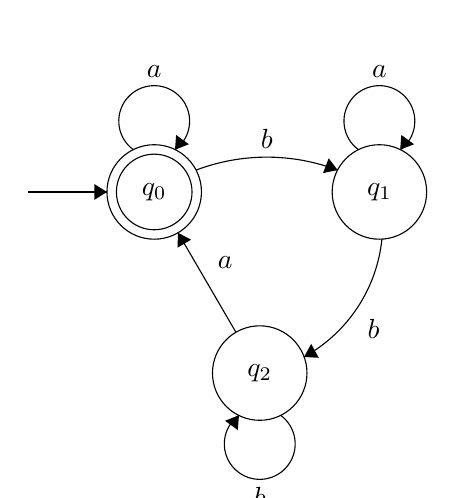
\begin{tikzpicture}[scale=0.2]
\tikzstyle{every node}+=[inner sep=0pt]
\draw [black] (30.6,-27) circle (3);
\draw (30.6,-27) node {$q_0$};
\draw [black] (30.6,-27) circle (2.4);
\draw [black] (44.9,-27) circle (3);
\draw (44.9,-27) node {$q_1$};
\draw [black] (37.3,-38.5) circle (3);
\draw (37.3,-38.5) node {$q_2$};
\draw [black] (22.6,-27) -- (27.6,-27);
\fill [black] (27.6,-27) -- (26.8,-26.5) -- (26.8,-27.5);
\draw [black] (29.277,-24.32) arc (234:-54:2.25);
\draw (30.6,-19.75) node [above] {$a$};
\fill [black] (31.92,-24.32) -- (32.8,-23.97) -- (31.99,-23.38);
\draw [black] (33.253,-25.614) arc (110.80524:69.19476:12.662);
\fill [black] (42.25,-25.61) -- (41.68,-24.86) -- (41.32,-25.8);
\draw (37.75,-24.29) node [above] {$b$};
\draw [black] (43.577,-24.32) arc (234:-54:2.25);
\draw (44.9,-19.75) node [above] {$a$};
\fill [black] (46.22,-24.32) -- (47.1,-23.97) -- (46.29,-23.38);
\draw [black] (45.061,-29.984) arc (-5.7922:-61.12681:9.674);
\fill [black] (40.11,-37.48) -- (41.05,-37.53) -- (40.57,-36.65);
\draw (44.12,-35.67) node [right] {$b$};
\draw [black] (35.79,-35.91) -- (32.11,-29.59);
\fill [black] (32.11,-29.59) -- (32.08,-30.54) -- (32.94,-30.03);
\draw (34.6,-31.51) node [right] {$a$};
\draw [black] (38.623,-41.18) arc (54:-234:2.25);
\draw (37.3,-45.75) node [below] {$b$};
\fill [black] (35.98,-41.18) -- (35.1,-41.53) -- (35.91,-42.12);
\end{tikzpicture}
\end{center}

	\item Suppose $M_1\neq M_2$ and $Q_1 = Q_2$ \\
	We can know that the $\delta_1 \neq \delta_2$ \\
	Therefore,  $\langle M_1 \rangle \neq \langle M_2 \rangle$\\
	And $\langle M \rangle$ is injective.

	\item We know that an encoding of a set $S$ is an injection function.\\
	and $\langle M \rangle \circ w =\langle M,w \rangle$\\
	Since $\langle M \rangle$ is injective,\\
	$\langle M,w \rangle: S\rightarrow \Omega^*$, and $\Omega = \{0, 1\}$ \\
	$w$ just states which input $M$ has for each transition. \\
	Therefore, $\langle M,w \rangle$ is an encoding.

	\item see Hw5-DFASimulatorTM
\end{enumerate}



\end{document}
